\pagestyle{fancy}
\setlength{\headheight}{16pt}
\fancyhead{} % clear all header fields
\fancyhead[L]{\textbf{TAM 514 Homework 4}}
\fancyhead[C]{Songyuan Cui}
\fancyhead[R]{\textbf{Spring 2025}}
\fancyfoot{} % clear all footer fields
\fancyfoot[C]{\thepage}

\begin{problem}
    \textbf{1 (100 pts).} Consider the following beam forced by a point force $P(t)$ applied at $x = x_1$ and a point moment $M(t)$ at $x = x_2$.
    The initial conditions are $u(x, t) = 0$ and $u_t(x, 0) = 0$.
    \begin{enumerate}[(i)]
        \item {
            Compute the orthonormalized vibration modes of this system and then compute analytically the response $u(x, t)$ of the beam using modal analysis.
        }
        \item {
            Now suppose that we want to  avoid exciting the second mode of the beam.
            Find the necessary and sufficient conditions for this to happen. 
            Find analytically the response $u(x, t)$ of the beam in that case.
        }
        \item Under what conditions can resonance occur in the system?
    \end{enumerate} 
\end{problem}
\begin{figure}[!ht]
    \centering
    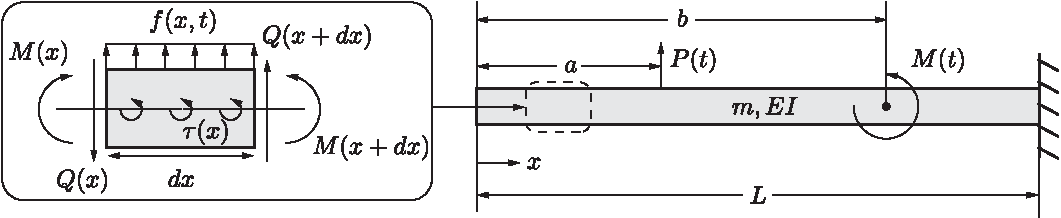
\includegraphics[width=\textwidth]{homework/hw4/assets/hw4_p1_setup.pdf}
\end{figure}
\begin{enumerate}[(i)]
\item { % 1(i)
    Consider the setup above and the free body diagram of a differential beam element of length $dx$. 
    Assume the arrows shown in the figure denote positive directions. 
    Here, the major departure from the lecture is the addition of a distributed external moment $\tau(x, t)$ defined similarly to the distributed force $f(x, t)$. 
    Based on assumptions made in class, the angular momentum balance on the differential element yields 
    \begin{equation}
        Q(x, t) = -\frac{\partial M}{\partial x}(x, t) - \tau(x, t)
    \end{equation}
    Given the constitutive relation $M(x, t) = EI u_{xx}(x, t)$, the equation of motion then reads
    \begin{equation}
    \begin{aligned}
        m \frac{\partial^2 u}{\partial t^2}(x, t) &= \frac{\partial Q}{\partial x}(x, t) + f(x, t) \\
        &= -\frac{\partial^2}{\partial x^2} \left[EI \frac{\partial^2 u}{\partial x^2}(x, t) \right] - \frac{\partial \tau}{\partial x}(x, t) + f(x, t)
    \end{aligned}
    \end{equation}
    In the case of the concentrated loads as shown in the figure, we leverage the Dirac delta function to define $f(x, t) = P(t)\delta(x - a)$ and $\tau(x, t) = M(t)\delta(x - b)$ (the notation $M(t)$ here is overloaded to represent the concentrated moment).
    The governing equation of the beam is then
    \begin{equation}\label{eqn:hw4_p1_gov_eqn}
        m \frac{\partial^2 u}{\partial t^2}(x, t) + EI \frac{\partial^4 u}{\partial x^4}(x, t) = P(t) \delta(x - a) - M(t) \frac{d \delta(x - b)}{dx}.
    \end{equation}
    Since the \emph{material coefficients are constant}, he boundary conditions are (free-clamped)
    \begin{equation}\label{eqn:hw4_p1_bc}
        \frac{\partial^2 u}{\partial x^2}(0, t) = 0, ~~~~ \frac{\partial^3 u}{\partial x^3}(0, t) = 0, ~~~~ u(L, t) = 0, ~~~~ \frac{\partial u}{\partial x}(L, t) = 0.
    \end{equation}
    Assume the separable ansatz $u(x, t) = \varphi(x) \eta(t)$, which is then substituted into the \emph{unforced} version of the governing equation \cref{eqn:hw4_p1_gov_eqn} to obtain 
    \begin{subequations}
    \begin{equation}\label{eqn:hw4_p1_space_eqn}
        EI \frac{d^4 \varphi}{dx^4}(x) = m \omega^2 \varphi(x),
    \end{equation}
    \begin{equation}
        \frac{d^2 \eta}{dt^2}(t) + \omega^2 \eta(t) = 0.
    \end{equation}
    \end{subequations} 
    Solving the spatial eigenvalue problem \cref{eqn:hw4_p1_space_eqn} yields solutions of the general form 
    \begin{equation}
        \varphi(x) = A \cos \frac{\sqrt{\omega}x}{\beta} + B \sin \frac{\sqrt{\omega}x}{\beta} + C \cosh \frac{\sqrt{\omega}x}{\beta} + D \sinh \frac{\sqrt{\omega}x}{\beta}, ~~~~ \beta = {\left(\frac{EI}{m}\right)}^{1/4}.
    \end{equation}
    Imposing the boundary conditions \cref{eqn:hw4_p1_bc} leads to the following system:
    \begin{equation}\label{eqn:hw4_p1_eigen}
        \begin{bmatrix}
            -1 & 0 & 1 & 0 \\
            0 & -1 & 0 & 1 \\
            \cos\mu & \sin\mu & \cosh\mu & \sinh\mu \\
            -\sin\mu & \cos\mu & \sinh\mu & \cosh\mu
        \end{bmatrix} \begin{bmatrix}
            A \\ B \\ C \\ D
        \end{bmatrix} = \begin{bmatrix}
            0 \\ 0 \\ 0 \\ 0
        \end{bmatrix}, ~~~~ \mu = \frac{\sqrt{\omega}L}{\beta}.
    \end{equation}
    Evidently, the first two equations lead to $A=C$ and $B=D$, which then leads to a simplified $2\times 2$ system 
    \begin{equation}\label{eqn:hw4_p1_eigen_simp}
        \underbrace{\begin{bmatrix}
            \cos\mu + \cosh\mu & \sin\mu + \sinh\mu \\
            -\sin\mu + \sinh\mu & \cos\mu + \cosh\mu
        \end{bmatrix}}_{\bt{A}} \begin{bmatrix}
            A \\ B
        \end{bmatrix} = \begin{bmatrix}
            0 \\ 0
        \end{bmatrix},
    \end{equation}
    which implies the imposing matrix $\bt{A}$ is singular:
    \begin{equation}
    \begin{aligned}
        0 &= \det(\bt{A}) = {(\cos\mu + \cosh\mu)}^2 - (\sinh^2\mu - \sin^2\mu) \\
        &= (\cos^2\mu + \sin^2\mu) + (\cosh^2\mu - \sinh^2\mu) + 2\cos\mu \cosh\mu \\
        &= 2(1 + \cos\mu \cosh\mu).
    \end{aligned}
    \end{equation}
    This leads to countably-infinite eigenvalues $\mu_n$ each satisfying $\boxed{1 + \cos\mu_n \cosh\mu_n = 0}$, graphically shown in \cref{fig:hw4_p1_evals} as intersections of $-\cos\mu$ and $1 / \cosh\mu$ ($\mu_1=1.8751,~\mu_2=4.6941,~\mu_3=7.8548,~\mu_4=10.9955,\ldots$). 
    For large $n$, the eigenvalues are approximately $\mu_n \approx (n-0.5)\pi$.
    The dimensional eigenvalues are obtained as $\boxed{\omega_n = {\left(\mu_n / L\right)}^2\sqrt{EI/m}}$.
    \begin{figure}[!ht]
        \centering
        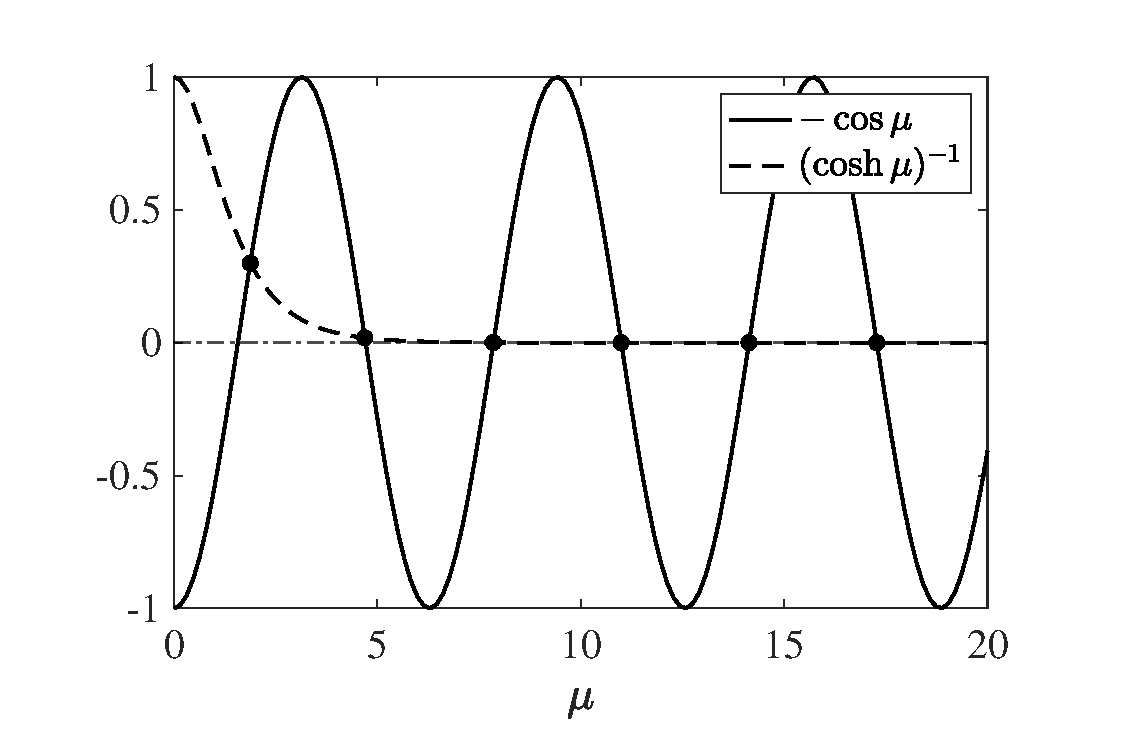
\includegraphics[width=0.5\textwidth]{homework/hw4/assets/hw4_p1_evals.pdf}
        \caption{
            Evaluation of eigenvalues $\mu_n$ as $x$-coordinates of intersections of $-\cos\mu$ and $1 / \cosh\mu$. 
            The intersections are marked in solid dots. 
            MATLAB code used to generate the figure can be found at \url{https://github.com/sy-cui/TAM514/blob/main/latex/homework/hw4/assets/hw4_p1.m}. 
        }\label{fig:hw4_p1_evals}
    \end{figure}
    
    The eigenvectors of the system \cref{eqn:hw4_p1_eigen,eqn:hw4_p1_eigen_simp} is a one-parameter ($A$) family satisfying
    \begin{equation}
        C_n = A_n, ~~~~ B_n = D_n = -\frac{\cos\mu_n + \cosh\mu_n}{\sin\mu_n + \sinh\mu_n} A_n, ~~~~ n = 1, 2, \ldots
    \end{equation}
    Hence, the mode shapes (eigenfunctions) are (for $n = 1, 2, \ldots$) 
    \begin{equation}\label{eqn:hw4_p1_spatial_soln}
        \boxed{\varphi_n(x) = A_n \left[\cos\frac{\mu_n x}{L} + \cosh\frac{\mu_n x}{L} - \frac{\cos\mu_n + \cosh\mu_n}{\sin\mu_n + \sinh\mu_n} \left(\cos\frac{\mu_n x}{L} + \cosh\frac{\mu_n x}{L}\right) \right]}
    \end{equation}
    To enforce mass-orthonormality, we require that $\int_0^L m \varphi_i(x) \varphi_j(x) dx = \delta_{ij}$ under simple boundary conditions (from lecture), which leads to 
    \begin{equation}\label{eqn:hw4_p1_coeff}
        \boxed{A_n = {\left\{ m \int_0^L {\left[\cos\frac{\mu_n x}{L} + \cosh\frac{\mu_n x}{L} - \frac{\cos\mu_n + \cosh\mu_n}{\sin\mu_n + \sinh\mu_n} \left(\cos\frac{\mu_n x}{L} + \cosh\frac{\mu_n x}{L}\right) \right]}^2 dx \right\}}^{-\frac{1}{2}}}
    \end{equation}
}
\item { % 1(ii)
    Under external loads, the temporal modal oscillators can be obtained by (1) writing the solution as a linear combination of eigenmodes $u(x, t) = \sum_{i=1}^\infty \varphi_i(x)\eta_i(t)$, (2) substituting into the governing equation \cref{eqn:hw4_p1_gov_eqn}, and (3) taking inner products with $\varphi_j(x)$ for some $j = 1, 2, \ldots$. 
    Leveraging mass/stiffness orthonormality, the temporal modal equations are obtained as 
    \begin{equation}\label{eqn:hw4_p1_temporal_eqn}
    \begin{aligned}
        \ddot{\eta}_j(t) + \omega_j^2 \eta_j(t) &= \int_0^L P(t) \delta(x - a) \varphi_j(x) dx - \int_0^L M(t) \frac{d\delta(x - b)}{dx} \varphi_j(x) dx \\
        &= P(t) \varphi_j(a) + M(t) \varphi_j'(b) \\ 
    \end{aligned}
    \end{equation}
    where we have used properties of the Dirac delta function:
    \begin{equation}
        \int_0^L \delta(x - a) f(x) dx = f(a), ~~~~ \int_0^L \frac{d\delta(x - b)}{dx} f(x) dx = -\frac{df}{dx}(b).
    \end{equation}
    The initial conditions, since $u(x, t) = 0$ and $u_t(x, 0)$, are simply $\eta_j(0) = 0$ and $\dot{\eta}_j(0) = 0$.
    Hence, the only source of modal oscillation is the forcing terms (and not the initial conditions). 
    In order to avoid exciting the second mode, we require that forcing be orthogonal to it, namely, 
    \begin{equation}
        \boxed{P(t) \varphi_2(a) + M(t) \varphi_2'(b) = 0}
    \end{equation}
    for all $t \geq 0$. Since $P(t)$ and $M(t)$ are arbitrary beyond the above conditions, we cannot solve \cref{eqn:hw4_p1_temporal_eqn} analytically and thus assume the solution to be $\eta_j(t)$ for $j = 1, 3, \ldots$.
    The normal mode solution is then 
    \begin{equation}
        \boxed{u(x, t) = \sum_{\substack{j=1 \\ j \neq 2}}^\infty \eta_j(t) \varphi_j(x)}
    \end{equation}
    with $\varphi_j(x)$ given in \cref{eqn:hw4_p1_spatial_soln,eqn:hw4_p1_coeff}.
}
\item { % 1(iii)
    Resonance occurs when the forcing contains sinusoidal components with driving frequency equal to at least one of the natural frequencies. 
    This is represented functionally as 
    \begin{equation}
        P(t) \varphi_j(a) + M(t) \varphi_j'(b) = \alpha \cos\omega_j t + \beta \sin\omega_j t,
    \end{equation}
    for some non-zero $\alpha$ and/or $\beta$ for at least one vibration mode $j = 1, 2, \ldots$.
}
\end{enumerate}

\newpage
\begin{problem}
    \textbf{2 (100 pts).} Consider the following beam with viscous damping: 
    \begin{equation}\label{eqn:hw4_p2_gov_eqn}
    \begin{gathered}
        u_{xxxx} + 4u_{xx} + 0.05 u_{t} + u_{tt} = 0, ~~~~ 0 \leq x \leq \pi, \\
        u(0, t) = u(\pi, t) = u_{xx}(0, t) = u_{xx}(\pi, t) = 0, ~~~~ u(x, 0) = f(x), ~~~~ u_t(x, 0) = g(x)\\
    \end{gathered}
    \end{equation}
    \begin{enumerate}[(i)]
        \item {
            Show that the following ansatz can be used to compute the response of this system 
            \begin{equation}\label{eqn:hw4_p2_ansatz}
                u(x, t) = \sum_{k=1}^{\infty}a_k(t) \sqrt{\frac{2}{\pi}} \sin kx
            \end{equation}
            and find the equations governing the modal amplitudes $a_k(t), ~k=1,2,\ldots$.
        }
        \item {
            Are all modes stable? 
            What is the physical mechanism that could cause instability? 
            Does the damping term affect the stability of the modes?
        }
        \item {
            Even if some of the modes prove to be unstable, is it possible that the overall response of the system to still be stable? 
            Under what conditions can this happen, and what is the expression of the stable response?
        }
    \end{enumerate}
\end{problem}
\begin{enumerate}[(i)]
\item { % 2(i)
    First, note that the boundary conditions in \cref{eqn:hw4_p2_gov_eqn} are readily satisfied by the ansatz \cref{eqn:hw4_p2_ansatz}, since $\sin k\pi = 0$ for $k = 1, 2, \ldots$. 
    Next, note the orthonormality condition:
    \begin{equation}
        \int_0^\pi \frac{2}{\pi}\sin nx \sin mx dx = \delta_{mn}
    \end{equation}
    Substituting the ansatz into the governing equation and taking inner products with $\sqrt{2/\pi}\sin jx$ yields
    \begin{equation}
    \begin{aligned}
        0 &= \frac{\pi}{2} \int_0^\pi \sin jx \left[\sum_{k=1}^\infty \left(k^4 a_k(t) \sin kx - 4k^2 a_k(t) \sin kx + 0.05 \dot{a}_k(t) \sin kx + \ddot{a}_k(t) \sin kx  \right) \right] dx \\
        &= \sum_{k=1}^\infty \delta_{jk} \left[\left(k^4 - 4k^2\right)a_k(t) + 0.05 \dot{a}_k(t) + \ddot{a}_k(t) \right] \\
        &= \ddot{a}_j(t) + 0.05 \dot{a}_j(t) + \left(j^4 - 4j^2\right)a_j(t)
    \end{aligned}
    \end{equation}
    which is independent of $x$ and decoupled with respect to the modes $j = 1, 2, \ldots$. 
    Hence, this proves that the separable ansatz \cref{eqn:hw4_p2_ansatz} is valid and leads to decoupled modal oscillators:
    \begin{equation}\label{eqn:hw4_p2_temporal_eqn}
        \boxed{\ddot{a}_k(t) + 0.05 \dot{a}_k(t) + \left(k^4 - 4k^2\right)a_k(t) = 0}, ~~~~ k = 1, 2, \ldots
    \end{equation}
}
\item { % 2(ii)
    The solution to the second-order linear constant-coefficient ODE \cref{eqn:hw4_p2_temporal_eqn} is of the exponential form $a_k(t) = A_k \exp (\omega_k t)$. 
    Assuming generic initial conditions, stability of the system requires that all exponents have no positive real part ($\real{\omega_k} \leq 0$).
    Substituting the exponential into \cref{eqn:hw4_p2_temporal_eqn} leads to the characteristic equation whose solution reads 
    \begin{equation}
        \omega_k = -\frac{1}{40} \left(1 \pm \sqrt{1 + 6400 k^2 - 1600 k^4} \right).
    \end{equation}
    for which we are only concerned when the negative sign is taken. 
    At $k = 1$, the root $\omega_1^{(2)} = (\sqrt{4801} - 1) / 40 > 0$ which implies instability. 
    For all other $k > 1$, the term $1 + 6400k^2 - 1600k^4 \leq 1$ and $\omega_k$ have non-positive real parts. 
    Thus, we conclude that \emph{the $k = 1$ mode is unstable, while all others are stable ($k = 2$ is quasi-stable / non-decaying)}. 

    This instability is caused by the negative tension term $4u_{xx}$. 
    If we remove the damping and flexural terms, the system becomes elliptical $4u_{xx} + u_{tt} = 0$ as opposed to hyperbolic in the case of the wave equation. 
    Physically, at $k = 1$ this term represents a negative tension (compression) imposed along the string / beam with mode shape $\sin(x)$.
    As time evolves, this mode leads to buckling behaviors, hence the instability.
 
    If we replace the damping coefficient $0.05$ with $\gamma$, the characteristic equation has solutions 
    \begin{equation}\label{eqn:hw4_p2_char_soln}
        \omega_k = \frac{1}{2}\left(-\gamma \pm \sqrt{\gamma^2 + 16k^2 - 4k^4} \right), ~~~~ k = 1, 2, \ldots
    \end{equation}
    for which we note that at $k = 1$, the larger root $\omega_1^{(2)} = (-\gamma + \sqrt{\gamma^2+12})/2 > 0$.
    This means that \emph{no matter what damping coefficient we use, the first mode will always be unstable}.
} 
\item { % 2(iii)
    Based on \cref{eqn:hw4_p2_char_soln}, we always have the first mode unstable, the second mode quasi-stable ($\omega_2^{(2)} = 0$), and all other modes stable. 
    Hence, given the initial conditions and external loads, \emph{the system will be stable if the first mode is never excited}. 
    Since there is no external loads in this case, we need only consider the initial conditions to \cref{eqn:hw4_p2_temporal_eqn}: 
    \begin{equation} \label{eqn:hw4_p2_ic}
        a_k(0) = \sqrt{\frac{2}{\pi}} \int_0^L f(x) \sin kx dx, ~~~~ \dot{a}_k(0) = \sqrt{\frac{2}{\pi}} \int_0^L g(x) \sin kx dx
    \end{equation}
    To never excite the first mode, we require that 
    \begin{equation}\label{eqn:hw4_p2_ic_1}
        \boxed{a_1(0) = \sqrt{\frac{2}{\pi}} \int_0^L f(x) \sin x dx = 0, ~~~~ \dot{a}_1(0) = \sqrt{\frac{2}{\pi}} \int_0^L g(x) \sin x dx = 0}
    \end{equation}
    which implies that $f(x)$ and $g(x)$ must be orthogonal to $\sin x$ over the interval $[0, L]$.

    For conciseness, we define $\gamma = 0.05$, $\Delta_k(\gamma) = \sqrt{\gamma^2 + 16k^2 - 4k^4}$, which leads to $\omega_k^{(1)} = -(\Delta_k+\gamma)/2$ and $\omega_k^{(2)} = (\Delta_k-\gamma)/2$. 
    Solving \cref{eqn:hw4_p2_temporal_eqn} with respect to initial conditions \cref{eqn:hw4_p2_ic} leads to the exponential solution 
    \begin{equation}
        a_k(t) = \frac{1}{2\Delta_k}\left\{\left[(\Delta_k - \gamma) a_k(0) - 2\dot{a}_k(0) \right]e^{-\frac{1}{2}(\Delta_k+\gamma)t} + \left[(\Delta_k + \gamma) a_k(0) + 2\dot{a}_k(0) \right]e^{\frac{1}{2}(\Delta_k-\gamma)t} \right\}
    \end{equation}
    valid for $k = 1, 2, 3, \ldots$. 
    Note that $a_1(t) \equiv 0$ under the required conditions \cref{eqn:hw4_p2_ic_1}. 
    Substitute into the ansatz \cref{eqn:hw4_p2_ansatz} to obtain the stable response of the system.
}
\end{enumerate}

\begin{problem}
    \textbf{3 (200 pts).} As a first step for computing the dynamical response of the following uniform simply supported beam with an attached two-DOF spring-mass oscillator, formulate and solve the eigenvalue problem and provide the orthonormality conditions for the eigenfunctions. 
    Then show how you can reduce the dynamics to an infinite set of uncoupled modal oscillators using modal analysis. 
    Discuss the local effect of the attachment, by considering the limiting cases $k \rightarrow 0$ and $k \rightarrow \infty$.
\end{problem}
\begin{figure}[!ht]
    \centering
    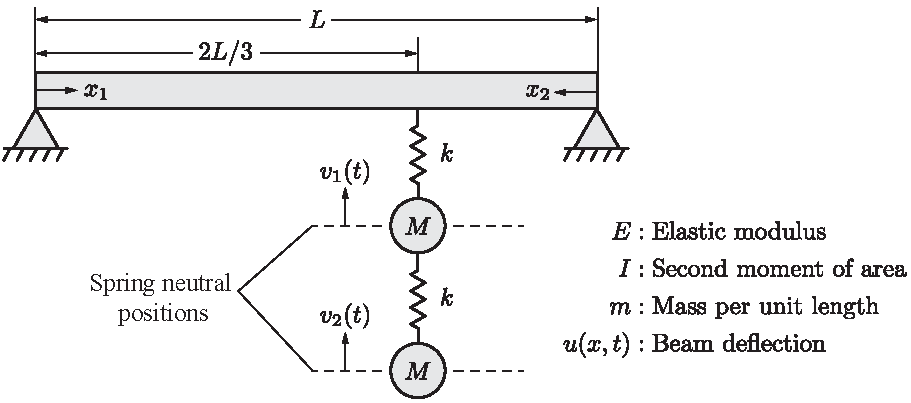
\includegraphics[width=0.7\textwidth]{homework/hw4/assets/hw4_p3_setup.pdf}
\end{figure}
Here, we separate the beam into two parts: one extending from the the left end to $x = 2L/3$, and the other extending from the right end ($x = L$) to $x = 2L/3$.
The two sub-beams use separate coordinates, with the left beam using $x_1 = x \in [0, 2L / 3]$ and the right beam using $x_2 = L - x \in [0, L / 3]$.
There displacement are denoted by $u_1(x_1, t)$ and $u_2(x_2, t)$, respectively.
The governing equations for the two beams and the two masses are 
\begin{subequations}\label{eqns:hw4_p3_gov_eqns}
\begin{equation}\label{eqn:hw4_p3_gov_eqn_beam1}
    m \frac{\partial^2 u}{\partial t^2}(x_1, t) + EI \frac{\partial^4 u}{\partial x_1^4}(x_1, t) = 0, ~~~~ x_1 \in \left[0, \frac{2L}{3}\right]
\end{equation}
\begin{equation}\label{eqn:hw4_p3_gov_eqn_beam2}
    m \frac{\partial^2 u}{\partial t^2}(x_2, t) + EI \frac{\partial^4 u}{\partial x_2^4}(x_2, t) = 0, ~~~~ x_2 \in \left[0, \frac{L}{3}\right]
\end{equation}
\begin{equation}
    M \frac{d^2v_1}{dt^2}(t) = k\left[u(a, t) - 2v_1(t) + v_2(t) \right]
\end{equation}
\begin{equation}
    M \frac{d^2v_2}{dt^2}(t) = k\left[v_1(t) - v_2(t) \right]
\end{equation}
\end{subequations}
for $t \geq 0$. 
A total of 8 boundary conditions are required for the two beam equations \cref{eqn:hw4_p3_gov_eqn_beam1,eqn:hw4_p3_gov_eqn_beam2}. 
Four are readily provided by the simply-supported ends, while the other four are enforced at their intersection ($x = 2L/3$): continuity in (1) displacement, (2) rotation, and (3) bending moment, as well as (4) the shear force balance.
(1) and (2) are due to the requirement that $u(x, t) \in \mathcal{C}^1$ for a beam. 
The bending moment is continuous at the intersection as the spring impose no additional moment, but it does contribute the shear forces.  
To form the shear force balance, we start from the static equation of the entire system and integrate in a small neighborhood of the intersection:
\begin{equation}
\begin{aligned}
    0 &= \frac{\partial Q}{\partial x}(x, t) - k\left[u\left(x, t\right) \delta\left(x - \frac{2L}{3}\right) - v_1(t)\right] \\
    &= \lim_{\epsilon\rightarrow 0} \int_{2L/3-\epsilon}^{2L/3+\epsilon} \left\{ \frac{\partial Q}{\partial x}(x, t) - k\left[u\left(x, t\right)  - v_1(t)\right]\delta\left(x - \frac{2L}{3}\right)\right\} dx \\
    &= \lim_{\epsilon\rightarrow 0} \left\{Q\left(\frac{2L}{3}+\epsilon, t\right) - Q\left(\frac{2L}{3}-\epsilon, t\right) - k\left[u\left(\frac{2L}{3}, t\right) - v_1(t)\right]\right\} \\
\end{aligned}
\end{equation}
Therefore, with constant material coefficients, the 8 boundary conditions read 
\begin{equation}\label{eqn:hw4_p3_bc}
\begin{gathered}
    u_1(0, t) = u_2(0, t) = 0, ~~~~ \frac{\partial^2 u_1}{\partial x_1^2}(0, t) = \frac{\partial^2 u_2}{\partial x_2^2}(0, t) = 0, \\
    u_1\left(\frac{2L}{3}, t\right) = u_2\left(\frac{L}{3}, t\right), ~~~~ \frac{\partial u_1}{\partial x_1}\left(\frac{2L}{3}, t\right) = -\frac{\partial u_2}{\partial x_2}\left(\frac{L}{3}, t\right), ~~~~ \frac{\partial^2 u_1}{\partial x_1^2}\left(\frac{2L}{3}, t\right) = \frac{\partial^2 u_2}{\partial x_2^2}\left(\frac{L}{3}, t\right), \\
    -EI\frac{\partial^3 u_1}{\partial x_1^3}\left(\frac{2L}{3}, t\right) + k\left[u_1\left(\frac{2L}{3}, t\right) - v_1(t) \right] = EI\frac{\partial^3 u_2}{\partial x_2^3}\left(\frac{L}{3}, t\right)
\end{gathered}
\end{equation}
In particular, we note that the partial derivative with respect to $x_2$ satisfies $\partial / \partial x_2 = - \partial/\partial x$.

Next, we perform modal analysis by assuming the separable ansatz 
\begin{equation}
    u_1(x_1, t) = \varphi^{(1)}(x_1) \eta(t), ~~~~ u_2(x_2, t) = \varphi^{(2)}(x_2) \eta(t), ~~~~ v_1(t) = \psi^{(1)} \eta(t), ~~~~ v_2(t) = \psi^{(2)} \eta(t)
\end{equation}
where $\psi^{(1)}$ and $\psi^{(2)}$ are scalars. 
After substituting the ansatz into the governing equations \cref{eqns:hw4_p3_gov_eqns}, we obtain the spatial modal eigenvalue problem 
\begin{subequations}\label{eqns:hw4_p3_spatial_eqns}
\begin{equation}\label{eqn:hw4_p3_spatial_eqn_beam1}
    EI \frac{d^4 \varphi^{(1)}}{dx_1^4}(x_1) = m \omega^2 \varphi^{(1)}(x_1), ~~~~ x_1 \in \left[0, \frac{2L}{3}\right]
\end{equation}
\begin{equation}\label{eqn:hw4_p3_spatial_eqn_beam2}
    EI \frac{d^4 \varphi^{(2)}}{dx_2^4}(x_2) = m \omega^2 \varphi^{(2)}(x_2), ~~~~ x_2 \in \left[0, \frac{L}{3}\right]
\end{equation}
\begin{equation}\label{eqn:hw4_p3_spatial_eqn_mass1}
    -\omega^2 M \psi^{(1)} = k\left[\varphi^{(1)}\left( \frac{2L}{3} \right) - 2 \psi^{(1)} + \psi^{(2)} \right]
\end{equation}
\begin{equation}\label{eqn:hw4_p3_spatial_eqn_mass2}
    -\omega^2 M \psi^{(2)} = k\left[\psi^{(1)} - \psi^{(2)} \right]
\end{equation}
\end{subequations}
where $\omega > 0$ represents the natural frequency of the system. 
The beam boundary conditions \cref{eqn:hw4_p3_bc} are then 
\begin{equation}\label{eqn:hw4_p3_spatial_bc}
\begin{gathered}
    \varphi^{(1)}(0) = \varphi^{(2)}(0) = 0, ~~~~ \frac{d^2 \varphi^{(1)}}{dx_1^2}(0) = \frac{d^2 \varphi^{(2)}}{dx_2^2}(0) = 0 \\
    \varphi^{(1)}\left(\frac{2L}{3}\right) = \varphi^{(2)}\left(\frac{L}{3}\right), ~~~~ \frac{d \varphi^{(1)}}{dx_1}\left(\frac{2L}{3}\right) = -\frac{d \varphi^{(2)}}{dx_2}\left(\frac{L}{3}\right), ~~~~ \frac{d^2 \varphi^{(1)}}{dx_1^2}\left(\frac{2L}{3}\right) = \frac{d^2 \varphi^{(2)}}{dx_2^2}\left(\frac{L}{3}\right) \\
    -EI\frac{d^3 \varphi^{(1)}}{dx_1^3}\left(\frac{2L}{3}\right) + k\left[\varphi^{(1)}\left(\frac{2L}{3}\right) - \psi^{(1)} \right] = EI\frac{d^3 \varphi^{(2)}}{dx_2^3}\left(\frac{L}{3}\right)
\end{gathered}
\end{equation}
The general solutions to \cref{eqn:hw4_p3_spatial_eqn_beam1,eqn:hw4_p3_spatial_eqn_beam2} are of the form
\begin{equation}
    \varphi^{(\alpha)}(x) = A^{(\alpha)} \cos \frac{\sqrt{\omega}x_\alpha}{\beta} + B^{(\alpha)} \sin \frac{\sqrt{\omega}x_\alpha}{\beta} + C^{(\alpha)} \cosh \frac{\sqrt{\omega}x_\alpha}{\beta} + D^{(\alpha)} \sinh \frac{\sqrt{\omega}x_\alpha}{\beta}, ~~~~ \beta = {\left(\frac{EI}{m}\right)}^{1/4},
\end{equation}
where $\alpha$ takes the indices $1, 2$ to shorthand notations for the two beams.
Due to the simply-supported boundary conditions (first row of \cref{eqn:hw4_p3_spatial_bc}), we have $A^{(1)} = A^{(2)} = C^{(1)} = C^{(2)} = 0$.
The four remaining boundary conditions at the interface, along with the equations of motion for the two masses \cref{eqn:hw4_p3_spatial_eqn_mass1,eqn:hw4_p3_spatial_eqn_mass2}, form a $6\times 6$ linear system:
\begin{equation}\label{eqn:hw4_p3_eigenvalue_problem}
    \underbrace{\begin{bmatrix}
        \sin 2\mu & \sinh 2\mu & -\sin \mu & -\sinh \mu & 0 & 0 \\
        \cos 2\mu & \cosh 2\mu & \cos \mu & \cosh \mu & 0 & 0 \\
        -\sin 2\mu & \sinh 2\mu & \sin \mu & -\sinh \mu & 0 & 0 \\
        \cos 2\mu+\kappa \sin 2\mu & - \cosh 2\mu + \kappa \sinh 2\mu & \cos \mu & -\cosh \mu & -\kappa & 0 \\
        -\sin 2\mu & -\sinh 2\mu & 0 & 0 & 2 - \omega^2 M/k & -1 \\
        0 & 0 & 0 & 0 & -1 & 1 - \omega^2 M/k
    \end{bmatrix}}_{\bt{A}}
    \begin{bmatrix}
        B^{(1)} \\ D^{(1)} \\ B^{(2)} \\ D^{(2)} \\ \psi^{(1)} \\ \psi^{(2)}
    \end{bmatrix} = 
    \begin{bmatrix}
        0 \\ 0 \\ 0 \\ 0 \\ 0 \\ 0
    \end{bmatrix}
\end{equation}
where we have defined two additional non-dimensional parameters:
\begin{equation}
    \mu(\omega) := \frac{\sqrt{\omega}L}{3\beta} = \frac{\sqrt{\omega} L}{3} {\left(\frac{m}{EI}\right)}^{\frac{1}{4}}, ~~~~ \kappa(\omega) := \frac{k\beta^3}{EI\omega^{\frac{3}{2}}} = \frac{k}{{\left(EIm^3 \omega^6 \right)}^{\frac{1}{4}}}
\end{equation}
A countably-infinite number of eigenvalues $\omega_i, ~i=1,2,\ldots$ can be obtained by setting $\det \bt{A} = 0$.
A representative plot of the determinants (absolute values) for arbitrarily chosen material parameters is shown in \cref{fig:hw4_p3_detA} (see the caption for details).
The eigenvectors (null space of $\bt{A}$) can also be determined up to a multiplicative constant, which we denote as 
\begin{equation}
    \bv{b}_i = c_i {\left[B^{(1)}_i ~D^{(1)}_i ~B^{(2)}_i ~D^{(2)}_i ~\psi^{(1)}_i ~\psi^{(2)}_i\right]}^T,
\end{equation}
where $c_i \in \mathbb{R}$ is free to be chosen. 
The eigenfunctions for the two sub-beams then read 
\begin{equation}
    \boxed{\varphi_i^{(\alpha)}(x) = c_i\left[B_i^{(\alpha)} \sin\frac{\sqrt{\omega_i}x_\alpha}{\beta} + D_i^{(\alpha)} \sinh\frac{\sqrt{\omega_i}x_\alpha}{\beta} \right]}, ~~~~ \alpha = 1, 2, ~~~~ i = 1, 2, \ldots.
\end{equation}
for which $x_1 \in [0, 2L/3]$ and $x_2 \in [0, L/3]$ concatenates the two functions to form a global eigenfunction over the interval $x \in [0, L]$.
\begin{figure}[!ht]
    \centering
    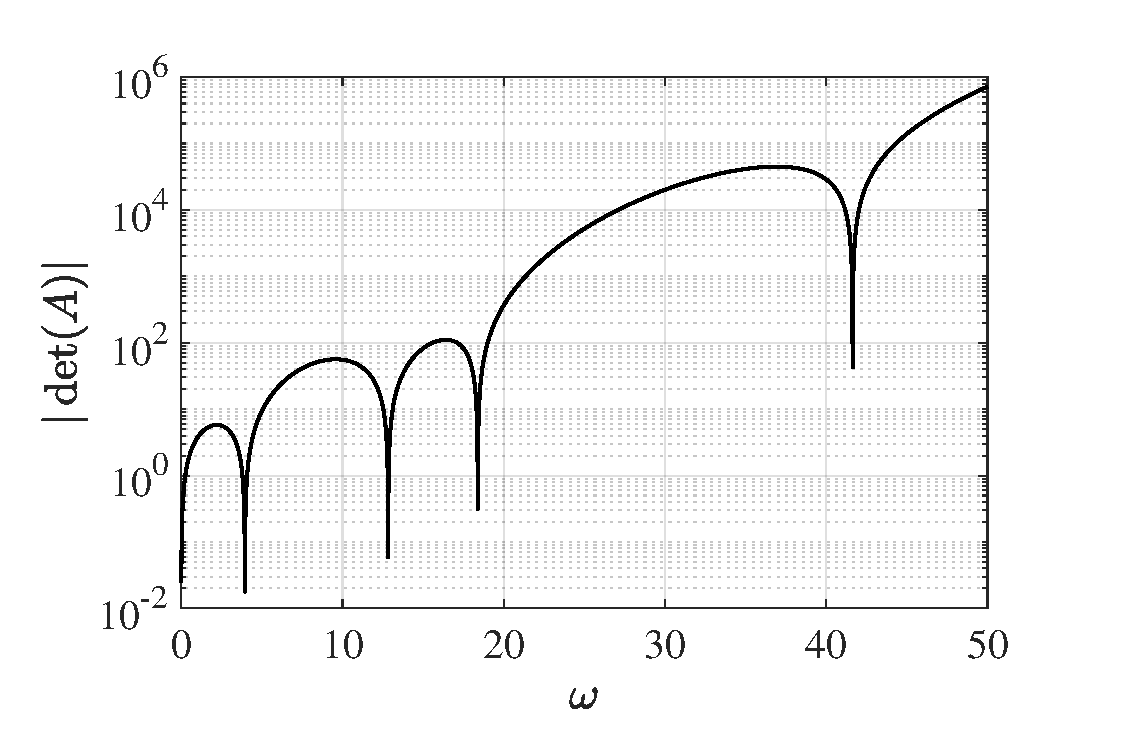
\includegraphics[width=0.6\textwidth]{homework/hw4/assets/hw4_p3_detA.pdf}
    \caption{
        Absolute value of the determinant ($| \det\bt{A} |$) plotted as a function of $\omega$.
        Due to the large magnitude of the determinant, the $y$-axis is plotted in log-scale, with each sharp valley representing the location of a natural frequency. 
        The material parameters are arbitrary chosen without dimensions: $EI = m = M = L = 1$, $k = 100$.
        MATLAB code used to generate this plot is provided at \url{https://github.com/sy-cui/TAM514/blob/main/latex/homework/hw4/assets/hw4_p3.m}.
    }\label{fig:hw4_p3_detA}
\end{figure}

To choose the coefficients $c_i$, we enforce the mass-orthonormality condition. 
Due to its connection with the kinetic energy of the system, we can directly write the condition as 
\begin{equation}\label{eqn:hw4_p3_mass_orthonormality}
    \boxed{\int_0^\frac{2L}{3} m \varphi_i^{(1)}(x_1) \varphi_j^{(1)}(x_1) dx_1 + \int_0^\frac{L}{3} m \varphi_i^{(2)}(x_2) \varphi_j^{(2)}(x_2) dx_2 + M \psi_i^{(1)} \psi_j^{(1)} + M \psi_i^{(2)} \psi_j^{(2)}= \delta_{ij},} ~~i,j = 1, 2, \ldots
\end{equation}
Nonetheless, a derivation of \cref{eqn:hw4_p3_mass_orthonormality} from the eigenproblem is provided below. 
\begin{prf}{}
Consider \cref{eqn:hw4_p3_spatial_eqn_beam1,eqn:hw4_p3_spatial_eqn_beam2} for the $i$-th mode. 
Taking inner products with the $j$-th mode in their respective domains, integrating by parts (4 times), and apply the simply-supported boundary conditions yield 
\begin{subequations}
\begin{equation}\label{eqn:hw4_p3_iprod_beam1}
\begin{aligned}
    \omega_i^2 \int_0^\frac{2L}{3} m \varphi_i^{(1)}(x_1) \varphi_j^{(1)}(x_1) dx_1 &= EI \int_0^\frac{2L}{3} \varphi_i^{(1)}(x_1) \frac{d^4 \varphi_j^{(1)}}{dx_1^4}(x_1) dx_1 \\ 
    & =  \omega_j^2 \int_0^\frac{2L}{3} m \varphi_i^{(1)}(x_1) \varphi_j^{(1)}(x_1) dx_1 + EI\left[\frac{d^3 \varphi_i^{(1)}}{dx_1^3} \varphi_j^{(1)} \right. \\
    &~~~ - \frac{d^2 \varphi_i^{(1)}}{dx_1^2} \frac{d \varphi_j^{(1)}}{dx_1}\left.+ \frac{d \varphi_i^{(1)}}{dx_1} \frac{d^2 \varphi_j^{(1)}}{dx_1^2} - \varphi_i^{(1)} \frac{d^3 \varphi_j^{(1)}}{dx_1^3}\right]_{x_1=\frac{2L}{3}}
\end{aligned}
\end{equation}
\begin{equation}\label{eqn:hw4_p3_iprod_beam2}
\begin{aligned}
    \omega_i^2 \int_0^\frac{L}{3} m \varphi_i^{(2)}(x_2) \varphi_j^{(2)}(x_2) dx_2 &= EI \int_0^\frac{L}{3} \varphi_i^{(2)}(x_2) \frac{d^4 \varphi_j^{(2)}}{dx_1^4}(x_2) dx_2 \\ 
    & =  \omega_j^2 \int_0^\frac{L}{3} m \varphi_i^{(2)}(x_2) \varphi_j^{(2)}(x_2) dx_2 + EI\left[\frac{d^3 \varphi_i^{(2)}}{dx_2^3} \varphi_j^{(2)} \right. \\
    &~~~ \left. - \frac{d^2 \varphi_i^{(2)}}{dx_2^2} \frac{d \varphi_j^{(2)}}{dx_2} + \frac{d \varphi_i^{(2)}}{dx_2} \frac{d^2 \varphi_j^{(2)}}{dx_2^2} - \varphi_i^{(2)} \frac{d^3 \varphi_j^{(2)}}{dx_2^3}\right]_{x_2=\frac{L}{3}}
\end{aligned}
\end{equation}
\end{subequations}
Adding \cref{eqn:hw4_p3_iprod_beam1,eqn:hw4_p3_iprod_beam2} and using the interfacial boundary conditions \cref{eqn:hw4_p3_spatial_bc} leads to
\begin{equation}
\begin{aligned}
    &~ \left(\omega_i^2 - \omega_j^2\right)\left[\int_0^\frac{2L}{3} m \varphi_i^{(1)}(x_1) \varphi_j^{(1)}(x_1) dx_1 + \int_0^\frac{L}{3} m \varphi_i^{(2)}(x_2) \varphi_j^{(2)}(x_2) dx_2\right] \\
    =&~
    EI\varphi_j^{(1)}\left(\frac{2L}{3}\right)\left[\frac{d^3 \varphi_i^{(1)}}{dx_1^3}\left(\frac{2L}{3}\right) + \frac{d^3 \varphi_i^{(2)}}{dx_2^3}\left(\frac{L}{3}\right)\right] - 
    EI\varphi_i^{(1)}\left(\frac{2L}{3}\right)\left[\frac{d^3 \varphi_j^{(1)}}{dx_1^3}\left(\frac{2L}{3}\right) + \frac{d^3 \varphi_j^{(2)}}{dx_2^3}\left(\frac{L}{3}\right)\right] \\
    =&~
    k\varphi_j^{(1)}\left(\frac{2L}{3}\right) \left[\varphi_i^{(1)}\left(\frac{2L}{3}\right) - \psi_i^{(1)}\right] - 
    k\varphi_i^{(1)}\left(\frac{2L}{3}\right) \left[\varphi_j^{(1)}\left(\frac{2L}{3}\right) - \psi_j^{(1)}\right] \\
    =&~
    k\varphi_i^{(1)}\left(\frac{2L}{3}\right) \psi_j^{(1)} - k\varphi_j^{(1)}\left(\frac{2L}{3}\right) \psi_i^{(1)}
\end{aligned}
\end{equation}
Notice that $\varphi_i^{(1)}(2L/3)$ can be written as a function of $\psi_i^{(1)}$ and $\psi_i^{(2)}$ using \cref{eqn:hw4_p3_spatial_eqn_mass1}:
\begin{equation}
\begin{aligned}
    &~ \left(\omega_i^2 - \omega_j^2\right)\left[\int_0^\frac{2L}{3} m \varphi_i^{(1)}(x_1) \varphi_j^{(1)}(x_1) dx_1 + \int_0^\frac{L}{3} m \varphi_i^{(2)}(x_2) \varphi_j^{(2)}(x_2) dx_2\right] \\
    =&~
    (2k - \omega_i^2 M)\psi_i^{(1)} \psi_j^{(1)} - k \psi_i^{(2)} \psi_j^{(1)} - 
    (2k - \omega_j^2 M)\psi_j^{(1)} \psi_i^{(1)} + k \psi_i^{(1)} \psi_j^{(2)}\\
    =&~
    \left(\omega_j^2 - \omega_i^2\right)M\psi_i^{(1)} \psi_j^{(1)} + (k - \omega_i^2 M) \psi_i^{(2)} \psi_j^{(2)} - (k - \omega_j^2 M) \psi_j^{(2)} \psi_i^{(2)} \\
    =&~ 
    \left(\omega_j^2 - \omega_i^2\right) 
    \left[M\psi_i^{(1)} \psi_j^{(1)} + M\psi_i^{(2)} \psi_j^{(2)}\right]    
\end{aligned}
\end{equation}
where in the second-to-last step we applied \cref{eqn:hw4_p3_spatial_eqn_mass2}. 
This proves that for $\omega_i \neq \omega_j$, we have mass-orthogonality
\begin{equation}
    \int_0^\frac{2L}{3} m \varphi_i^{(1)}(x_1) \varphi_j^{(1)}(x_1) dx_1 + \int_0^\frac{L}{3} m \varphi_i^{(2)}(x_2) \varphi_j^{(2)}(x_2) dx_2 + M \psi_i^{(1)} \psi_j^{(1)} + M \psi_i^{(2)} \psi_j^{(2)} = 0
\end{equation}
Hence, the mass-orthonormality is indeed enforced by \cref{eqn:hw4_p3_mass_orthonormality}, which in turn determines the coefficients $c_i$.
\end{prf}

Up to this point, we have determined the eigenvalues ($\omega_i$) and associated spatial modes ($\varphi_i^{(1)}(x_1)$, $\varphi_i^{(2)}(x_2)$, $\psi_i^{(1)}$, and $\psi_i^{(2)}$) of the system.
To find the modal oscillator equations, we write the solutions as linear combinations of the eigenfunctions:
\begin{equation}
    u_1(x, t) = \sum_{i=1}^\infty \varphi_i^{(1)}(x) \eta_i(t), ~~~~
    u_2(x, t) = \sum_{i=1}^\infty \varphi_i^{(2)}(x) \eta_i(t), ~~~~ 
    v_1(t) = \sum_{i=1}^\infty \psi_i^{(1)} \eta_i(t), ~~~~ 
    v_2(t) = \sum_{i=1}^\infty \psi_i^{(2)} \eta_i(t).
\end{equation}
Substitute into \cref{eqns:hw4_p3_gov_eqns}, take inner products, and utilize the spatial modal equations \cref{eqns:hw4_p3_spatial_eqns} to obtain 
\begin{subequations}
\begin{align}
\begin{split}\label{eqn:hw4_p3_temporal_eqn_beam1}
    0 &= \sum_{i=1}^\infty \ddot{\eta}_i(t) \int_0^{\frac{2L}{3}} m \varphi_i^{(1)} (x_1) \varphi_j^{(1)}(x_1) dx_1 + \sum_{i=1}^\infty \eta_i(t) \int_0^{\frac{2L}{3}} EI \frac{d^4\varphi_i^{(1)}}{dx_1^4} \varphi_j^{(1)}(x_1) dx_1 \\
    &= \sum_{i=1}^\infty \left[\ddot{\eta}_i(t) + \omega_i^2 \eta_i(t) \right] \int_0^{\frac{2L}{3}} m \varphi_i^{(1)} (x_1) \varphi_j^{(1)}(x_1) dx_1 
\end{split}\\
\begin{split}\label{eqn:hw4_p3_temporal_eqn_beam2}
    0 &= \sum_{i=1}^\infty \ddot{\eta}_i(t) \int_0^{\frac{L}{3}} m \varphi_i^{(2)} (x_2) \varphi_j^{(2)}(x_2) dx_2 + \sum_{i=1}^\infty \eta_i(t) \int_0^{\frac{L}{3}} EI \frac{d^4\varphi_i^{(2)}}{dx_2^4} \varphi_j^{(2)}(x_2) dx_2 \\
    &= \sum_{i=1}^\infty \left[\ddot{\eta}_i(t) + \omega_i^2 \eta_i(t) \right] \int_0^{\frac{L}{3}} m \varphi_i^{(2)} (x_2) \varphi_j^{(2)}(x_2) dx_2
\end{split}\\
\begin{split}\label{eqn:hw4_p3_temporal_eqn_mass1}
    0 &= \sum_{i=1}^\infty M \ddot{\eta}_i(t) \psi_i^{(1)} \psi_j^{(1)} - \sum_{i=1}^\infty k\eta_i(t) \left[\varphi_i^{(1)}\left(\frac{2L}{3}\right) - 2\psi_i^{(1)} + \psi_i^{(2)} \right] \psi_j^{(1)} \\
    &= \sum_{i=1}^\infty M \left[\ddot{\eta}_i(t) + \omega_i^2 \eta_i(t) \right]  \psi_i^{(1)} \psi_j^{(1)}
\end{split}\\
\begin{split}\label{eqn:hw4_p3_temporal_eqn_mass2}
    0 &= \sum_{i=1}^\infty M \ddot{\eta}_i(t) \psi_i^{(2)} \psi_j^{(2)} - \sum_{i=1}^\infty k\eta_i(t) \left[\psi_i^{(1)} - \psi_i^{(2)}\right] \psi_j^{(2)} \\
    &= \sum_{i=1}^\infty M \left[\ddot{\eta}_i(t) + \omega_i^2 \eta_i(t) \right]  \psi_i^{(2)} \psi_j^{(2)}
\end{split}
\end{align}
\end{subequations}
Adding all four equations (\cref{eqn:hw4_p3_temporal_eqn_beam1,eqn:hw4_p3_temporal_eqn_beam2,eqn:hw4_p3_temporal_eqn_mass1,eqn:hw4_p3_temporal_eqn_mass2}) into one and using the mass-orthonormality condition \cref{eqn:hw4_p3_mass_orthonormality} leads to the temporal modal oscillators:
\begin{equation}
    \boxed{\ddot{\eta}_i(t) + \omega_i^2 \eta_i(t) = 0}, ~~~~ i = 1, 2, \ldots
\end{equation}

As $k \rightarrow 0$, the matrix $\bt{A}$ becomes (almost) block-diagonal, suggesting that the beam and the masses are (almost) decoupled.
In particular, the beam behaves like a simply-supported beam whose eigenmodes are sine functions, and the masses' modes on the leading order are stationary (since there are effectively no spring connecting them). 

As $k \rightarrow \infty$, the influence of $M$ almost vanishes, and on the leading order the eigenproblem \cref{eqn:hw4_p3_eigenvalue_problem} becomes 
\begin{equation}
    \det \begin{bmatrix}
        \sin 2\mu & \sinh 2\mu & -\sin \mu & -\sinh \mu & 0 & 0 \\
        \cos 2\mu & \cosh 2\mu & \cos \mu & \cosh \mu & 0 & 0 \\
        -\sin 2\mu & \sinh 2\mu & \sin \mu & -\sinh \mu & 0 & 0 \\
        \sin 2\mu & \sinh 2\mu & 0 & 0 & -1 & 0 \\
        0 & 0 & 0 & 0 & 1 & -1 \\
        0 & 0 & 0 & 0 & -1 & 1 \\
    \end{bmatrix} = 0
\end{equation}
which leads to $\psi^{(1)} = \psi^{(2)}$ (the two masses are in sync). 
The same applies to the beam at the position where it is attached to the spring-mass system. 
This suggests that the beam forfeits its shear stress continuity at that location and instead enforces an additional fixed-position condition. 

\newpage
\begin{problem}
    \textbf{4 (200 pts).} Formulate Rayleigh's quotient for these two beam systems, labelled System \Rom{1} and System \Rom{2}. 
    Then develop a discretized numerical methodology (either Rayleigh-Ritz or Galerkin) to approximately solve the resulting eigenvalue problems. 
    Assign your own (reasonable!) numerical values in SI metric system to the system parameters and find approximations for the first three modes of these systems (i.e., approximations to the natural frequencies and mode shapes). 
    Under what conditions the dynamics of System \Rom{1} can resemble a two-DOF system?
\end{problem}
\begin{figure*}[!ht]
    \centering
    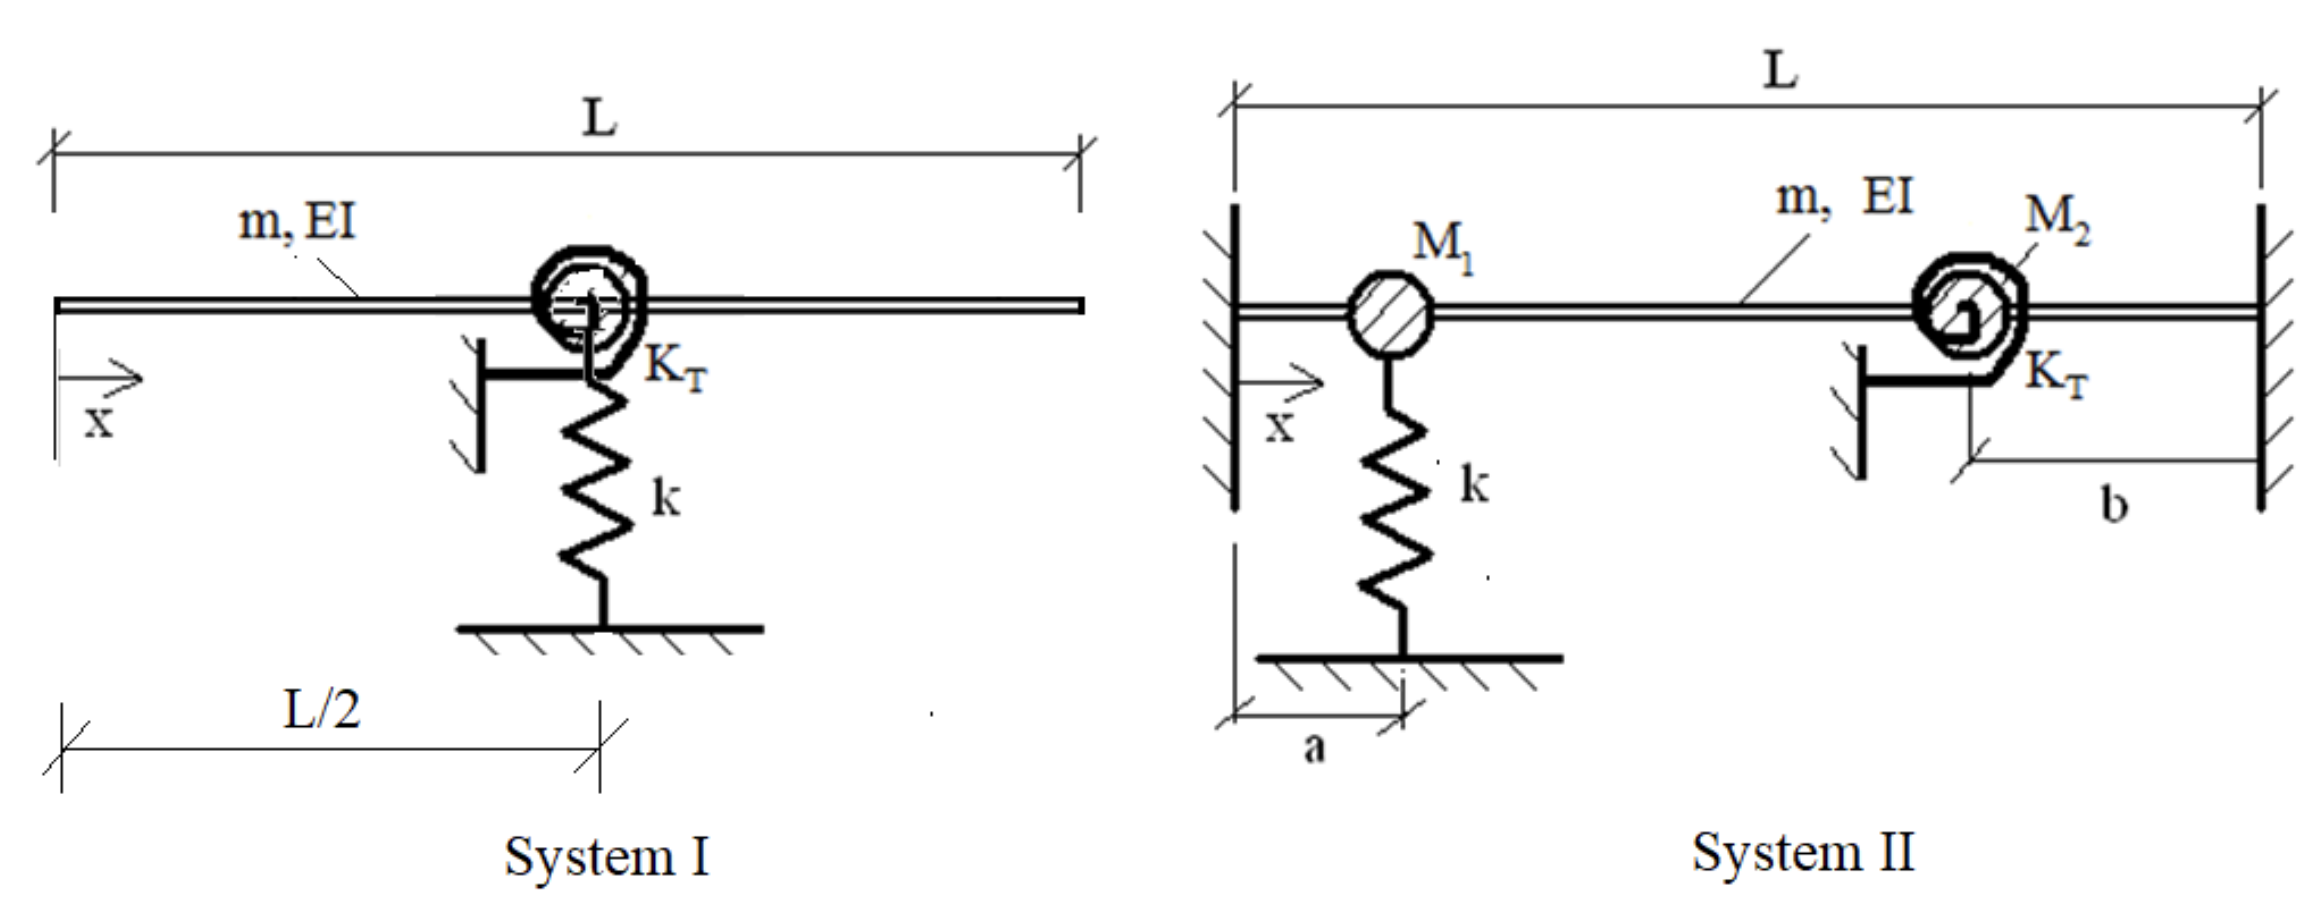
\includegraphics[width=\linewidth]{homework/hw4/assets/hw4_p4_setup.png}
\end{figure*}
The Rayleigh quotient for a given admissable trial function $\tilde{\varphi}_i(x)$ is the ratio between the potential and kinetic energy associated with the trial function.
Hence, for system \Rom{1}, the Rayleigh quotient reads
\begin{equation}
    \mathcal{R}_{\Rom{1}}[\tilde{\varphi}_i(x)] = \frac{ 
        \int_0^L EI {\tilde{\varphi}_i''(x)}^2 dx + k {\tilde{\varphi}_i(L/2)}^2 + K_T {\tilde{\varphi}_i'(L/2)}^2
    }{
        \int_0^L m {\tilde{\varphi}_i(x)}^2 dx 
    }
\end{equation}
and for system \Rom{2}:
\begin{equation}
    \mathcal{R}_{\Rom{2}}[\tilde{\varphi}_i(x)] = \frac{ 
        \int_0^L EI {\tilde{\varphi}_i''(x)}^2 dx + k {\tilde{\varphi}_i(a)}^2 + K_T {\tilde{\varphi}_i'(L-b)}^2
    }{
        \int_0^L m {\tilde{\varphi}_i(x)}^2 dx + M_1 {\tilde{\varphi}_i(a)}^2 + M_2 {\tilde{\varphi}_i(L-b)}^2
    }
\end{equation}
To approximate the eigenmodes, we employ the same approach as the previous assignment where we use Lagrangian polynomials as basis functions to compose the trial function:
\begin{equation}\label{eqn:hw4_p4_lagrangian}
    \tilde{\varphi}(x) = \sum_{j=0}^N u_j l_j(x), ~~~~ l_j(x) = \hat{l}_j(\xi) = \prod_{\substack{i=0 \\ i\neq j}}^N \frac{\xi - \xi_i}{\xi_j - \xi_i}, ~~~~ \xi(x) = \frac{2}{L}x - 1
\end{equation} 
and $\xi_i$ are Gauss-Legendre-Lobatto nodes on the $[-1, 1]$ interval.
This leads to the mass and stiffness matrices of the two systems, which in index notation ($i, j = 0, 1, \ldots N$) read 
\begin{equation}
\begin{aligned}
    M_{ij}^{\Rom{1}} &= \int_0^L m l_i(x) l_j(x) dx \\
    K_{ij}^{\Rom{1}} &= \int_0^L EI l_i''(x) l_j''(x) dx + k l_i(L/2) l_j(L/2) + K_T l_i'(L/2) l_j'(L/2) \\
    M_{ij}^{\Rom{2}} &= \int_0^L m l_i(x) l_j(x) dx + M_1 l_i(a) l_j(a) + M_2 l_i(L-b) l_j(L-b) \\
    K_{ij}^{\Rom{2}} &= \int_0^L EI l_i''(x) l_j''(x) dx + k l_i(a) l_j(a) + K_T l_i'(L-b) l_j'(L-b)
\end{aligned}
\end{equation}
The eigenproblem is then $\bt{K}\bv{u}_i = \omega_i^2 \bt{M} \bv{u}_i$ where $\omega_i$ is the $i$-th eigenvalue / natural frequency, and $\bv{u}_i \in \mathbb{R}^{N+1}$ contains the coefficients $u_j$ of the $i$-th mode and must satisfy the boundary conditions. 
For system \Rom{1}, both boundaries are free and thus there is no constraint on $\bv{u}_i$. 
For system \Rom{2}, both boundaries are clamped and thus the following must be satisfied 
\begin{equation}
    u_0 = u_N = 0, ~~~~ \sum_{j=0}^N u_j l_j'(\xi(0)) = \sum_{j=0}^N u_j l_j'(\xi(L)) = 0.
\end{equation}
The first (Dirichlet) condition can be satisfied by defining a restriction / prolongation matrix $\bt{R}$ such that
\begin{equation}
    \bt{R}\bv{u} = \bt{R} \begin{bNiceArray}{c}[margin]
        u_0 \\ 
        u_1 \\  
        \vdots\\
        u_{N-1} \\
        u_N 
    \end{bNiceArray} = \begin{bNiceArray}{c}[margin]
        u_1 \\  
        \vdots\\
        u_{N-1} \\
    \end{bNiceArray} = \tilde{\bv{u}}, ~~~~ \bv{R}^T \tilde{\bv{u}} = \begin{bNiceArray}{c}[margin]
        0 \\ 
        u_1 \\  
        \vdots\\
        u_{N-1} \\
        0
    \end{bNiceArray}
\end{equation} 
In other words, the transpose action of this matrix prolongates the internal nodes to have boundary values of zeros.
The second (Neumann) condition, however, requires additional treatment. 
Here, we elect to use Lagrangian multipliers $\bv{\lambda} = {[\lambda_1, \lambda_2]}^T$, and define a constraint matrix $\bv{C} \in \mathbb{R}^{2\times(N-1)}$ such that 
\begin{equation}
    C_{1i} = l_i'(\xi(0)), ~~~~ C_{2i} = l_i'(\xi(L)), ~~~~ i = 1, \ldots, N-1.
\end{equation}
where we do not need the indices $i=0$ and $i = N$ as we already have $u_0 = u_N = 0$.
The eigenvalue problem for system \Rom{2} is then augmented to
\begin{equation}
    \begin{bmatrix}
        \bt{R} \bt{K}^{\Rom{2}} \bt{R}^T & \bt{C}^T \\
        \bt{C} & 0
    \end{bmatrix}
    \begin{bmatrix}
        \tilde{\bv{u}} \\ \bv{\lambda}
    \end{bmatrix} = 
    \omega^2 
    \begin{bmatrix}
        \bt{R} \bt{M}^{\Rom{2}} \bt{R}^T & 0 \\
        0 & 0
    \end{bmatrix}
    \begin{bmatrix}
        \tilde{\bv{u}} \\ \bv{\lambda}
    \end{bmatrix}
\end{equation}
This system is singular and may be difficult to solve. 
Instead we may use a nullspace projection technique where we find an orthonormal basis of $\bt{C}$'s nullspace $\bt{Q} \in \mathbb{R}^{(N-1)\times (N-3)}$ such that 
\begin{equation}
    \bt{C} \bt{Q} = \bt{0} \in \mathbb{R}^{2\times(N-3)}, ~~~~ \bt{Q}^T \bt{Q} = \bt{I} \in \mathbb{R}^{(N-3)\times(N-3)}
\end{equation}
Computationally, $\bt{Q}$ can be obtained by performing a QR factorization on $\bt{C}^T$ and removing the first two column of the orthogonal matrix. 
Since the solution $\tilde{u}$ must be in the nullspace of $\bt{C}$, there exists a unique $\bv{v} \in \mathbb{R}^{N-3}$ such that $\bv{u} = \bt{Q} \bv{v}$, which then transforms the eigenvalue problem to 
\begin{equation}
    \left( \bt{Q}^T \bt{R} \bt{K}^{\Rom{2}} \bt{R}^T \bt{Q} \right) \bv{v} = \omega^2 \left( \bt{Q}^T \bt{R} \bt{M}^{\Rom{2}} \bt{R}^T \bt{Q} \right) \bv{v}
\end{equation}

For both systems, we assume an aluminum beam of length $\qty{1}{\m}$ and square cross-section of side $\qty{0.1}{\m}$. 
All parameters are listed in \cref{tab:hw4_p4_params}.
For the polynomial order, we choose $N = 10$ (i.e. 11th-degree polynomials). 
The corresponding mass-orthonormalized nodal coefficients $u_j$ are tabulated in \cref{tab:hw4_p4_coeffs} for the first three modes, and the synthesized eigenfunctions are plotted in \cref{fig:hw4_p4_efunc}, \emph{with flexibility in the choice of signs}.
\begin{table}[!ht]
    \centering
    \begin{tabular}{|c|c|c|c|c|c|c|c|c|c|}
        \hline
        $L$ & $E$ & $I$ & $m$ & $k$ & $K_T$ & $M_1$ & $M_2$ & $a$ & $b$ \\
        \hline
        \qty{1}{m} & \qty{70}{GPa} & \qty{8.33e-6}{m^4} & \qty{27}{kg/m} & \qty{2e3}{N/m} & \qty{e3}{N} & \qty{10}{kg} & \qty{15}{kg} & \qty{0.2}{m} & \qty{0.3}{m} \\
        \hline
    \end{tabular}
    \caption{Geometry and material parameters for both systems.}\label{tab:hw4_p4_params}
\end{table}

\begin{table}[!ht]
    \centering
    \begin{tabular}{|c|c|c|c|c|c|c|}
        \hline
        & \multicolumn{3}{c|}{System \Rom{1}} & \multicolumn{3}{c|}{System \Rom{2}} \\ \hline
        $u_0$ & 0.1925 & 0.3333 & 0.3849 & 0 & 0 & 0 \\ \hline
        $u_1$ & 0.1925 & 0.3113 & 0.3259 & 0.0139 & 0.0425 & 0.0460 \\ \hline
        $u_2$ & 0.1925 & 0.2615 & 0.1931 & 0.1290 & 0.3748 & 0.3457 \\ \hline
        $u_3$ & 0.1925 & 0.1884 & 0.0104 & 0.4177 & 0.9321 & 0.4497 \\ \hline
        $u_4$ & 0.1924 & 0.0986 & -0.1615 & 0.7784 & 1.0204 & -0.4817 \\ \hline
        $u_5$ & 0.1924 & -0.0000 & -0.2340 & 0.9891 & 0.3412 & -1.0290 \\ \hline
        $u_6$ & 0.1924 & -0.0986 & -0.1615 & 0.8816 & -0.4470 & -0.1225 \\ \hline
        $u_7$ & 0.1925 & -0.1884 & 0.0104 & 0.5061 & -0.5365 & 0.4704 \\ \hline
        $u_8$ & 0.1925 & -0.2615 & 0.1931 & 0.1592 & -0.2100 & 0.2490 \\ \hline
        $u_9$ & 0.1925 & -0.3113 & 0.3259 & 0.0172 & -0.0249 & 0.0330 \\ \hline
        $u_10$ & 0.1925 & -0.3333 & 0.3849 & 0 & 0 & 0 \\
        \hline
    \end{tabular}
    \caption{Nodal coefficients for the first three modes of both systems. }\label{tab:hw4_p4_coeffs}
\end{table}


\begin{figure}[!ht]
    \centering
    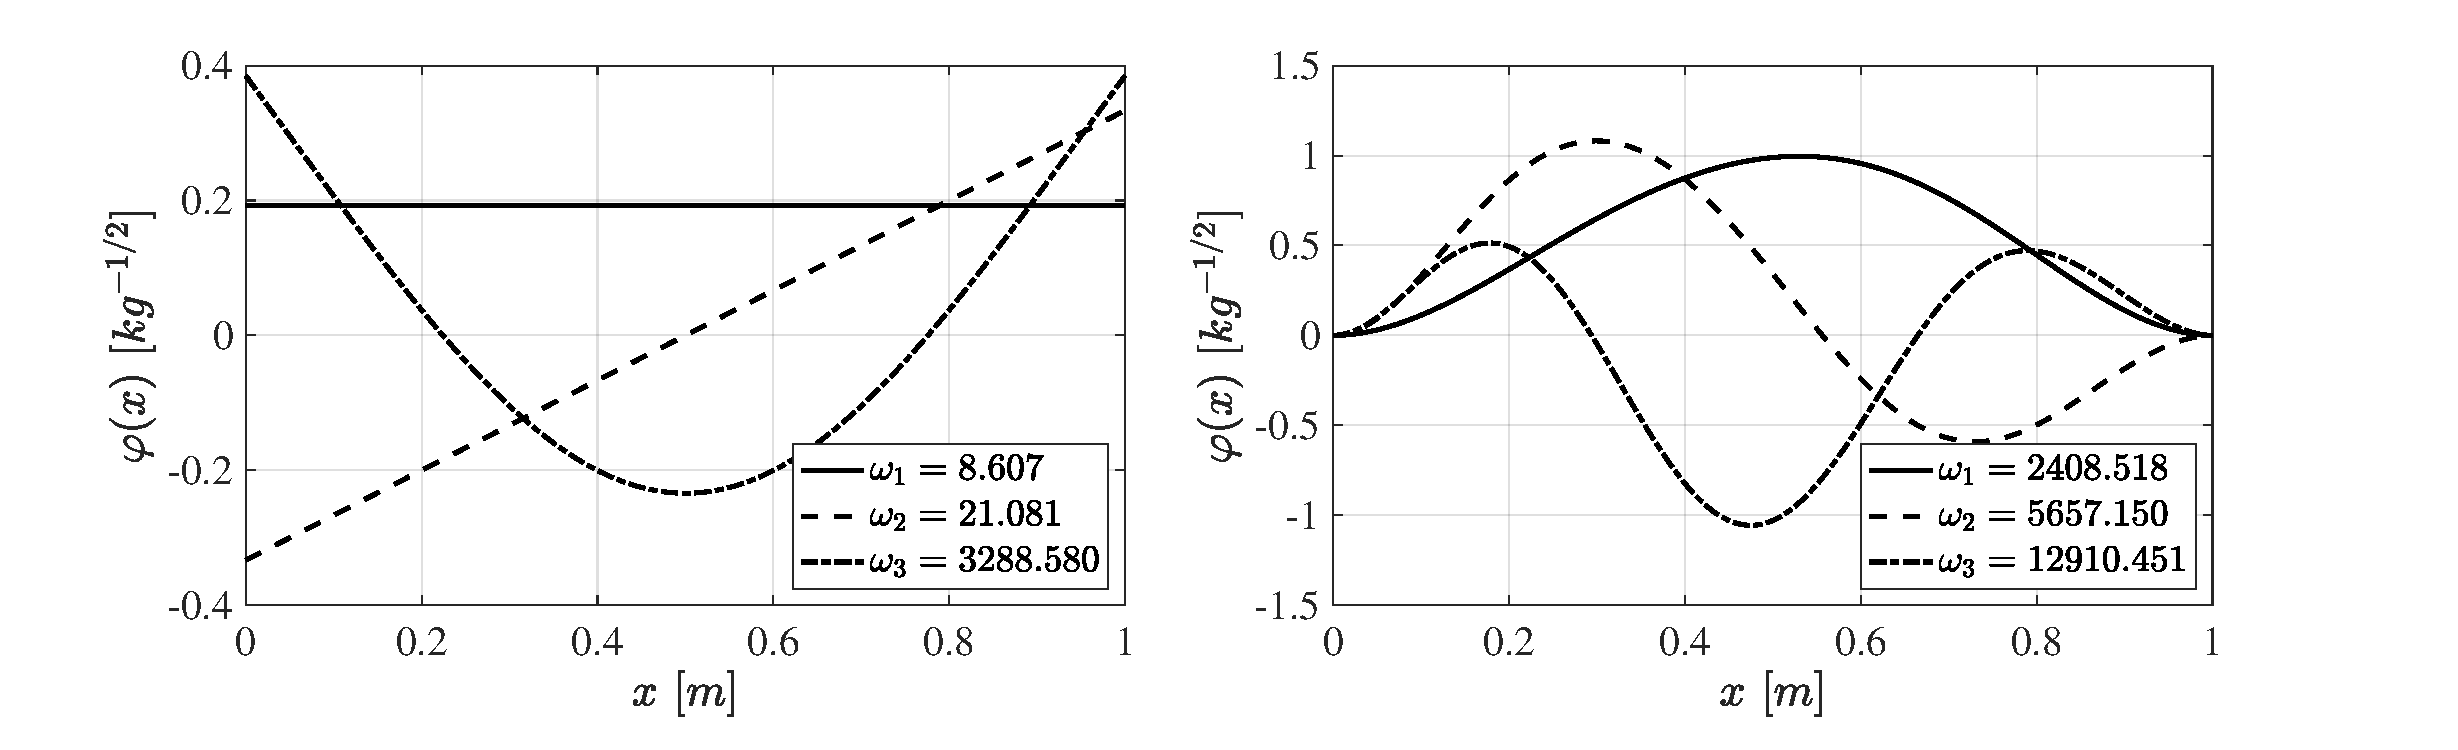
\includegraphics[width=\textwidth]{homework/hw4/assets/hw4_p4_efunc.pdf}
    \caption{
        First three mass-orthonormalized eigenfunctions and eigenvalues for System \Rom{1} (left) and System \Rom{2} (right). 
        The functions are synthesized using \cref{eqn:hw4_p4_lagrangian} with coefficients tabulated in \cref{tab:hw4_p4_coeffs}. 
        MATLAB code used to generate this plot, as well as the data in \cref{tab:hw4_p4_coeffs}, is provided at \url{https://github.com/sy-cui/TAM514/blob/main/latex/homework/hw4/assets/hw4_p4.m}.
    }\label{fig:hw4_p4_efunc}
\end{figure}

\noindent\textbf{\emph{Under what conditions
the dynamics of System I can resemble a two-DOF system?}}

Here the two degrees of freedom refer to the the displacement and rotation at the connection point, namely $u(L/2, t)$ and $u_x(L/2, t)$. 
If the system resembles a two-DOF system, then it implies that the beam behaves almost rigidly, with displacement and rotation conforming to the linear and torsional springs. 
Based on \cref{fig:hw4_p4_efunc} (left), the first two eigenmodes have significantly lower natural frequencies and have eigenfunctions that are close to a horizontal line and linear function, respectively.
The horizontal line encodes rigid-like translation, and the linear function (constant slope) encodes rigid-like rotation.
Hence, for the entire system to behave like a two-DOF system, we require $k \rightarrow \infty$ and $K_T \rightarrow \infty$, which would set the first two natural frequencies close to the spring-mass frequencies. 